\documentclass[a4paper, UKenglish, cleveref, autoref, thm-restate]{lipics-v2021}
%This is a template for producing LIPIcs articles. 
%See lipics-v2021-authors-guidelines.pdf for further information.
%for A4 paper format use option "a4paper", for US-letter use option "letterpaper"
%for british hyphenation rules use option "UKenglish", for american hyphenation rules use option "USenglish"
%for section-numbered lemmas etc., use "numberwithinsect"
%for enabling cleveref support, use "cleveref"
%for enabling autoref support, use "autoref"
%for anonymousing the authors (e.g. for double-blind review), add "anonymous"
%for enabling thm-restate support, use "thm-restate"
%for enabling a two-column layout for the author/affilation part (only applicable for > 6 authors), use "authorcolumns"
%for producing a PDF according the PDF/A standard, add "pdfa"

%\pdfoutput=1 %uncomment to ensure pdflatex processing (mandatatory e.g. to submit to arXiv)
%\hideLIPIcs  %uncomment to remove references to LIPIcs series (logo, DOI, ...), e.g. when preparing a pre-final version to be uploaded to arXiv or another public repository

%\graphicspath{{./graphics/}}%helpful if your graphic files are in another directory

% Determine whether it is local compilation or overleaf compilation
\makeatletter
\begingroup\endlinechar=-1\relax
       \everyeof{\noexpand}%
       \edef\x{\endgroup\def\noexpand\homepath{%
         \@@input|"kpsewhich --var-value=HOME" }}\x
\makeatother
\def\overleafhome{/tmp}% change as appropriate

\bibliographystyle{plainurl}% the mandatory bibstyle
\usepackage{float}


\usepackage{amsmath} % need to be on top for eps files
\usepackage{mathtools}

\usepackage{graphicx}

\usepackage{cleveref}

\usepackage{algorithmicx}

\usepackage{algcompatible}
\crefname{algocf}{alg.}{algs.}
\Crefname{algocf}{Algorithm}{Algorithms}
\usepackage[ruled,vlined,linesnumbered]{algorithm2e}
\usepackage[ruled,vlined,linesnumbered]{algorithm2e}
\renewcommand{\algorithmiccomment}[1]{\bgroup\hfill\tiny//~#1\egroup}
\newcommand\bigO[1]{$\mathcal{O}(#1)$}

\crefname{lstlisting}{listing}{listings}
\Crefname{lstlisting}{Listing}{Listings}

\title{WhitePaper: Cyber-Security Variant of TruCol protocol} %TODO Please add
\subtitle{Eliminating triage intermediaries for zero-day exploits using a decentralised payout protocol}
%\titlerunning{Spiking Minimum Dominating Set Approximation} %TODO optional, please use if title is longer than one line

%\titlerunning{Dummy short title} %TODO optional, please use if title is longer than one line
% TODO: remove names from print for double blind article
\author{Chihab Amghane}{Radboud University}%, [optional: Address], Country \and My second affiliation, Country \and \url{http://www.myhomepage.edu} }
{}{}{(Optional) author-specific funding acknowledgements}%TODO mandatory, please use full name; only 1 author per \author macro; first two parameters are mandatory, other parameters can be empty. Please provide at least the name of the affiliation and the country. The full address is optional

\author{Victoria Bosch}{Radboud University}%, [optional: Address], Country \and My second affiliation, Country \and \url{http://www.myhomepage.edu} }
{}{}{}%TODO mandatory, please use full name; only 1 author per \author macro; first two parameters are mandatory, other parameters can be empty. Please provide at least the name of the affiliation and the country. The full address is optional

\author{Rashim Charles}{Radboud University}%, [optional: Address], Country \and My second affiliation, Country \and \url{http://www.myhomepage.edu} }
{}{}{}%TODO mandatory, please use full name; only 1 author per \author macro; first two parameters are mandatory, other parameters can be empty. Please provide at least the name of the affiliation and the country. The full address is optional

\author{Marc Droogh}{Delft University of Technology}%, [optional: Address], Country \and My second affiliation, Country \and \url{http://www.myhomepage.edu} }
{}{}{}%TODO mandatory, please use full name; only 1 author per \author macro; first two parameters are mandatory, other parameters can be empty. Please provide at least the name of the affiliation and the country. The full address is optional

\author{Clara Maine}{Radboud University}%, [optional: Address], Country \and My second affiliation, Country \and \url{http://www.myhomepage.edu} }
{}{}{}%TODO mandatory, please use full name; only 1 author per \author macro; first two parameters are mandatory, other parameters can be empty. Please provide at least the name of the affiliation and the country. The full address is optional

\author{Chinari Subhechha Subudhi}{Delft University of Technology}%, [optional: Address], Country \and My second affiliation, Country \and \url{http://www.myhomepage.edu} }
{}{}{}%TODO mandatory, please use full name; only 1 author per \author macro; first two parameters are mandatory, other parameters can be empty. Please provide at least the name of the affiliation and the country. The full address is optional

\author{Akke Toeter}{Delft University of Technology, Radboud University}%, [optional: Address], Country \and My second affiliation, Country \and \url{http://www.myhomepage.edu} }
{a.h.h.toeter@student.tudelft.nl}{0000-0002-9577-920X}{}%TODO mandatory, please use full name; only 1 author per \author macro; first two parameters are mandatory, other parameters can be empty. Please provide at least the name of the affiliation and the country. The full address is optional

\author{Eric van der Toorn}{Delft University of Technology}%, [optional: Address], Country \and My second affiliation, Country \and \url{http://www.myhomepage.edu} }
{}{}{}%TODO mandatory, please use full name; only 1 author per \author macro; first two parameters are mandatory, other parameters can be empty. Please provide at least the name of the affiliation and the country. The full address is optional

% \author{V Bosch}{Radboud}{email}{[orcid]}

% \author{A Diehl}{Radboud}{email}{[orcid]}

% \author{A Toeter}{Radboud}{email}{[orcid]}

% \author{Kwisthout}{Radboud}{email}{[orcid]}


\authorrunning{ } %TODO mandatory. First: Use abbreviated first/middle names. Second (only in severe cases): Use first author plus 'et al.'

\Copyright{ } %TODO mandatory, please use full first names. LIPIcs license is "CC-BY";  http://creativecommons.org/licenses/by/3.0/

\ccsdesc[500]{Computing methodologies~Distributed algorithms}
\ccsdesc[500]{Computer systems organization~Neural networks}

% \ccsdesc[100]{\textcolor{red}{Replace ccsdesc macro with valid one}} %TODO mandatory: Please choose ACM 2012 classifications from https://dl.acm.org/ccs/ccs_flat.cfm 

\keywords{Cyber-security, bounties, zero-day exploits, decentralised technology} %TODO mandatory; please add comma-separated list of keywords

\category{} %optional, e.g. invited paper

\relatedversion{} %optional, e.g. full version hosted on arXiv, HAL, or other respository/website
%\relatedversiondetails[linktext={opt. text shown instead of the URL}, cite=DBLP:books/mk/GrayR93]{Classification (e.g. Full Version, Extended Version, Previous Version}{URL to related version} %linktext and cite are optional

%\supplement{}%optional, e.g. related research data, source code, ... hosted on a repository like zenodo, figshare, GitHub, ...
%\supplementdetails[linktext={opt. text shown instead of the URL}, cite=DBLP:books/mk/GrayR93, subcategory={Description, Subcategory}, swhid={Software Heritage Identifier}]{General Classification (e.g. Software, Dataset, Model, ...)}{URL to related version} %linktext, cite, and subcategory are optional

%\funding{(Optional) general funding statement \dots}%optional, to capture a funding statement, which applies to all authors. Please enter author specific funding statements as fifth argument of the \author macro.

\acknowledgements{I want to thank \dots}%optional

% \nolinenumbers %uncomment to disable line numbering

\graphicspath{{latex/publication_opodis_2021/images/}}


%Editor-only macros:: begin (do not touch as author)%%%%%%%%%%%%%%%%%%%%%%%%%%%%%%%%%%
\EventEditors{Akke Toeter}
\EventNoEds{2}
\EventLongTitle{}
\EventShortTitle{TruSec}
\EventAcronym{}
\EventYear{2021}
\EventDate{December 23, 2021}
\EventLocation{Delft, Nijmegen}
\EventLogo{}
\SeriesVolume{2}
\ArticleNo{2}
%%%%%%%%%%%%%%%%%%%%%%%%%%%%%%%%%%%%%%%%%%%%%%%%%%%%%%

\begin{document}
% Comment.
\maketitle

\ifx\homepath\overleafhome
% Overleaf compilation.
    \section{Introduction}
\label{sec:introduction}
This document presents a Trustless Security protocol that aims to help ethical hackers retrieve zero-day exploit bounties without ambiguity, whilst simultaneously enabling companies to show their customers how much money is staked on their open source software stacks.


To explain how the protocol may help both of these stakeholders (ethical hackers and companies using open source software), we will first describe, what we think is, a typical procedure for vulnerability disclosures in \cref{sec:assumptions}. Then we will explain how the protocol can improve upon that in \cref{sec:protocol}. Next, \cref{sec:implementation} describes strategies to specify how the protocol may be implemented. The limitations and weaknesses of our strategy and protocol are detailed in \cref{sec:discussion}. This white-paper is concluded in \cref{sec:conclusion}.
    \section{Assumptions}\label{sec:assumptions}
This section present some of the assumptions that are made about the current way zero-day exploits, and vulnerabilities in general are treated.

\subsection{Ethical Hacker Perspective}
\begin{enumerate}
	\item We assume it is not always as easy and/or attractive for whitehat hackers/ethical hackers to publish an exploit and retrieve an accompanying financial reward for the publication. This assumption is based on popular media such as darknet diaries, posts on \url{news.ycombinator.com}, communications with two ethical hackers and possibly other sources. This assumption is based on (a combination of) the following sub-assumptions:
	\begin{enumerate}
		\item Vulnerabilities may be discovered at small/non-profit software development companies that have not allocated a large budget fraction to security.
		\item Ambiguity in the specification of the bug bounty/reward program may be interpreted in the advantage of the company during triage.
		\item The triage process may take a relatively long time, requiring the ethical hacker to have sufficient funds to sustain living costs coverage until the pay-out.
		\item A conservative/carefulness in the ethical hacker towards approaching the company with respect to the legality of discovering the vulnerability may hinder/slow down the vulnerability disclosure process.
		\item The effort required to contact the company and convince them of the seriousness of the bug may consume unnecessary resources.
	\end{enumerate}
\end{enumerate}

\subsection{Company - perspective}
\begin{enumerate}
	\item We assume cybersecurity vulnerabilities become increasingly more relevant in our increasingly more digitized world. This assumption may be seen as being substantiated by for example the \textit{Cyber Security Assessment Netherlands 2021 (CSAN 2021)} as presented by the Dutch National Coordinator Counterterrorism and Safety of the Ministry of Justice and Security. Currently, there is only the Dutch version available at: \url{https://www.nctv.nl/onderwerpen/cybersecuritybeeld-nederland/documenten/publicaties/2021/06/28/cybersecuritybeeld-nederland-2021}. We assume that this trend can be extrapolated from a Dutch perspective to a more global perspective, given the international media coverage of many ransomware attacks.
	\item We assume that companies are interested, or will become more interested, in showing their customers and/or stakeholders (a quantified perspective on) \textit{how} secure their technology is. We assume it can be quite challenging to convey this perspective clearly due to the following factors:
	\begin{enumerate}
		\item Vulnerabilities can be found in various sections of the company, ranging from social engineering, misconfiguration to zero-day exploits. It is difficult to give customers a comprehensive yet concise/simple insight in how "secure" all these attack surfaces are.
		\item The impact of a vulnerability may be ambiguous or not easily quantifiable. For example, for some companies, vulnerabilities may allow malicious actors to take over critical infrastructure, whilst other vulnerabilities may lead to data leaks or other undesired side effects.
		\item It may be difficult to accurately assess the capabilities of malicious adversaries.
	\end{enumerate}
	\item We assume some companies might be unfamiliar with vulnerability disclosure and accompanying triage processes. These delicate processes may seem intimidating for new companies that want to start paying attention to their cybersecurity, and this may lead to a lower allocation of cybersecurity budget.
\end{enumerate}
    \section{Protocol}
\label{sec:protocol}

    \section{Implementation}\label{sec:implementation}

    \section{Discussion}
\label{sec:discussion}
The presented proposal for protocol development can be critically evaluated. This section aims to identify possible weak points.
\subsection{Limitations}
The following limitations are identified in the protocol:
\begin{enumerate}
    \item The proposed protocol, in its initial form, does not (necessarily) work for security compromises that are not clearly pre-defined. For example, if the decentralised virtual machine/stack/honeypot is configured to only pay-out in case an internal value/secret is modified, a whitehat hacker might be able to gain read-access to the secret, which could be considered a hack, but the whitehat hacker would not receive a payout. Accordingly, companies may specify different payouts to different types of security breaches. This may reduce the added value of collaborative staking.
    \item The running a decentralised virtual machine with a high degree of decentralisation, along with their interactions is expected to be costly. This expectation is based on approximate costs of roughly 50 dollars for a single Ethereum transaction \cite{todo}.
    \item We expect most hacks do not rely on pure zero-day exploits, accordingly we think the scope of this protocol is significantly limited w.r.t. the complete cybersecurity threat landscape.
    \item This protocol will most likely not allow companies to test their entire system, as we currently consider it practically infeasible to simulate the various types of social engineering and or interactions with non-decentralised platforms (on a blockchain). So companies cannot, in good conscience, make claims about their overall level of cybersecurity based on this protocol alone.
    \item This protocol does not protect against economically irrational malicious agents. Examples could be:
    \begin{enumerate}
        \item Actors with revenge sentiment. They could for example skip the payout and use zero-day exploits to hurt a company that staked their open source software stack.
        \item Nation states may not care about payouts and instead use found zero-day exploits themselves, instead of disclosing them.
    \end{enumerate}
\end{enumerate}

\subsection{Related Work}
It was noted during the TechEx conference, that companies like Google and Microsoft already fund vulnerability disclosures for, for example, Ubuntu. This can be seen as collective funding, hence one could argue the added value of the proposed protocol may be limited in this respect.

Additionally, there are companies like HackerOne that perform independent triage, hence one could argue the added value of doing this in a decentralised fashion is limited.%\newpage
    \section{Conclusion and Recommendations}
\label{sec:conclusion}
The proposed protocol can enable companies to convey a quantitative level of security of (segments of) their open source technology stack their customers. Customers can use this information on the minimum price for zero-day exploit, and compare it to their costs of suffering from a malicious zero-day exploit. This may allow them to (re)allocate their funds and cyber-security resources based on the accompanying risk-profile. 

The Additionally, the protocol enables whitehat/ethical hackers to retrieve payouts directly without ambiguity.

Since computational budgets typically are costly on decentralised computing platforms, a recommendation is included to ,
%% Summarize the other chapters
%% Explain what TruSec does

%% Write how TruSec works
%% Summarise implementation
%% Summarize security issues
%% Summarise discussion
%% Mention the protocol can promote a fair and inclusive TDD market contributing to SDG 8.



%\subsection{Recommendations}
%% Include the possible impact of the protocol on society
%The following recommendations are made:
%\begin{enumerate}[label=\arabic*]
    %% To mitigate edge cases
%    \item \label{rec:ecosystem} 
%    \item \label{rec:prelauch_period}
%    \item \label{rec:security_tools}
%\end{enumerate}
\else
% Local compilation
    \section{Introduction}
\label{sec:introduction}
This document presents a Trustless Security protocol that aims to help ethical hackers retrieve zero-day exploit bounties without ambiguity, whilst simultaneously enabling companies to show their customers how much money is staked on their open source software stacks.


To explain how the protocol may help both of these stakeholders (ethical hackers and companies using open source software), we will first describe, what we think is, a typical procedure for vulnerability disclosures in \cref{sec:assumptions}. Then we will explain how the protocol can improve upon that in \cref{sec:protocol}. Next, \cref{sec:implementation} describes strategies to specify how the protocol may be implemented. The limitations and weaknesses of our strategy and protocol are detailed in \cref{sec:discussion}. This white-paper is concluded in \cref{sec:conclusion}.
    \section{Assumptions}\label{sec:assumptions}
This section starts with the assumptions that we made about the way vulnerability disclosures of zero-day exploits are currently typically handled.

\subsection{Ethical Hacker Perspective}
\begin{enumerate}
	\item We assume it is not always convenient and beneficial for ethical hackers to publish an exploit and retrieve an accompanying financial reward. This assumption is based on private communications with two ethical hackers %TODO: include footnote.
	and popular media such as darknet diaries, posts on \url{news.ycombinator.com},  and possibly other sources. % TODO: find publication that identifies satisfiablitiy of hackers with cybersecurity bug bounty programs/triage processes.
	This assumption is based on (a combination of) the following sub-assumptions:
	\begin{enumerate}
		\item If ethical hackers give a complete disclosure of the vulnerability directly to the company, they lose their negotiating leverage. A trusted triage intermediary is often used to overcome this issue.
		\item The effort required to contact the company and convince them of the seriousness of the bug may consume unnecessary resources.
		\item Cautiousness from the ethical hacker with respect to the legality of discovering the vulnerability when approaching the company  may hinder/slow down the vulnerability disclosure process.
		\item Ambiguity in the specification of the bug bounty/reward program may be interpreted in the advantage of the company during triage.
		\item The triage process may take a relatively long time, requiring the ethical hacker to have sufficient funds to sustain living costs coverage until the pay-out.
		\item The triage intermediary consumes financial resources, which lower the amount allocatable to the hacker, and/or raise the cost of cyber-security defences.
		\item Vulnerabilities may be discovered at small/non-profit software development companies that have not allocated a large budget fraction to security. This may render navigating the vulnerability disclosure process succesfully, challenging for such small/non-profit organisation.
	\end{enumerate}
\end{enumerate}

\subsection{Company Perspective}
\begin{enumerate}
	\item We assume cybersecurity vulnerabilities become increasingly more relevant in our increasingly more digitized world. This assumption may be seen as being substantiated by for example the \textit{Cyber Security Assessment Netherlands 2021 (CSAN 2021)} as presented by the Dutch National Coordinator Counterterrorism and Safety of the Ministry of Justice and Security. Currently, there is only the Dutch version available at: \url{https://www.nctv.nl/onderwerpen/cybersecuritybeeld-nederland/documenten/publicaties/2021/06/28/cybersecuritybeeld-nederland-2021}. We assume that this trend can be extrapolated from a Dutch perspective to a more global perspective, given the international media coverage of many ransomware attacks.
	\item We assume that companies are interested, or will become more interested, in showing their customers and/or stakeholders (a quantified perspective on) \textit{how} secure their technology is. We assume it can be quite challenging to convey this perspective clearly due to the following factors:
	\begin{enumerate}
		\item Vulnerabilities can be found in various sections of the company, ranging from social engineering, misconfiguration to zero-day exploits. It is difficult to give customers a comprehensive yet concise/simple insight in "how secure" each of these attack surfaces are.
		\item The impact of a vulnerability may be ambiguous or not easily quantifiable. For example, for some companies, vulnerabilities may allow malicious actors to take over critical infrastructure, whilst other vulnerabilities may lead to data leaks or other undesired side effects.
		\item It may be difficult to accurately assess the capabilities of malicious adversaries.
	\end{enumerate}
	\item We assume some companies might be unfamiliar with vulnerability disclosure and accompanying triage processes. These delicate processes may seem intimidating for new companies that want to start paying attention to their cybersecurity, and this may lead to a lower allocation of cybersecurity budget.
\end{enumerate}
    \section{Protocol}
\label{sec:protocol}
This section presents the TruSec protocol, and explains how it can improve the way vulnerability disclosures are completed for deterministically verifiable zero-day exploits.

\subsection{Scope}\label{subsec:scope}
The protocol is primarily designed to automate deterministically verifiable zero-day exploits vulnerability disclosures. It can also be used to hedge against misconfigurations and supply-chain attacks. For example, companies can add a specific configuration (yaml) to the DVM, and add a bounty on that forked DVM. This way, a hacker may leverage the particular configuration to find an exploit. This procedure also allows the protocol to identify some supply-chain attack vulnerabilities. For example, if an invalid certificate is used to compromise the device.

However, both misconfiguration and supply chain attack partially deviate from the main benefit of collective nature of the protocol. For example, it may incentivise hackers to focus efforts on particular configurations, that are not (necessarily) useful for other companies. However, at the same time, hackers could still opt to focus on the mutual elements of all forked decentralised virtual machines (DVMs) to collect the bounties with a single, more powerful exploit. This scope/applicability of the protocol is visualised in \cref{fig:protocol_scope}.
\begin{figure}[H]
    \centering
    \ifx\homepath\overleafhome
        \includegraphics[width=0.50\textwidth]{Images/Diagrams/scope.png}
    \else
        \includegraphics[width=0.50\textwidth]{latex/Images/Diagrams/scope.png}
    \fi
    \caption{The proposed TruSec protocol is not suited to deal with social engineering attacks, nor is it ideal for misconfiguration exploits and/or supply-chain attacks. Instead, it is designed to increase the rate of discovery of deterministically verifiable zero-day exploits. Note, we acknowledge that attacks can be, and often are, a combination of the types.}
    \label{fig:protocol_scope}
\end{figure}
With respect to \cref{fig:protocol_scope}, the following notes are made:
\begin{enumerate} 
    \item The orange attack types imply the proposed protocol is not designed to tackle these issues, nor does it provide full coverage (against malicious agents) for these attack types. However:
    \begin{enumerate}
        \item The misconfiguration could be covered if companies upload their configurations into DVMs. These configurations would typically not benefit from the collaborative staking, as it is less likely that other companies happen to use the same configurations.
        \item Some of the supply chain attacks could be covered if the ethical hackers are able to propagate these supply chain exploits into the DVMs.
    \end{enumerate}
\end{enumerate}

\subsection{Usage}
\noindent With this scope defined, one can look at how companies and ethical hackers interact according to the proposed protocol.

\noindent The basic idea is that companies and users (stakeholders) can put their open source software stacks on a decentralised virtual machine DVM. They can then collectively stake money on the security of the stacks, such that everyone can see how much money says: \textit{the use of certain software packages/combinations is safe}. This enables companies, to show their customers for example:

\noindent \textit{With us, your data is stored using MongoDB Version 5.1, \$314.159,- says it is uncompromised, and it's running on Ubuntu Server version 21.10, which has \$4.200.000,- staked on its security. This setup has a configuration with a security on which we staked \$9001,-. If any of these software packages get compromised by ethical hackers, \underline{we will be the first to know.}}

\noindent We believe that might be clear language that enables decision makers and customers interested in company $A$, to get a simple, and intuitive understanding on: \textit{how secure} is the software stack of company A?

\noindent For the ethical/ethical hackers, the advantages are clear; they know before they start their work how large their payout will be, and they get a direct payout upon completion of their work (after the predetermined responsible disclosure period has ended).

\subsubsection{Disclaimer}
The presented protocol does not provide insight in the complete security of a system/company. As visualised in \cref{fig:protocol_scope}, the protocol does not cover all attack surfaces of companies. Hence, if other attack surfaces, such as social engineering are used, companies can still get compromised, regardless of the amount they staked. Therefore, it is important that the numerical value of the amount staked on the zero-day exploit security level is not abused to convey a false sense of security by the staking companies to their customers.

\subsection{Description}
The protocol is shown in \cref{fig:interaction}.
\begin{figure}[H]
    \centering
    \ifx\homepath\overleafhome
        \includegraphics[width=1.0\textwidth]{Images/Diagrams/interaction.png}
    \else
        \includegraphics[width=1.0\textwidth]{latex/Images/Diagrams/interaction.png}
    \fi
    
    \caption{Visualisation of the interaction of the TruSec protocol. This is an ever-lasting cycle, where at the end of the process, companies can re-deploy the patched decentralised stack, and allocate new funds. ethical hackers can scan for new attacks.}
    \label{fig:interaction}
\end{figure}
\noindent 

\noindent To summarize, the protocol enables companies and users of open source software to collectively stake money on the software stacks of their choice. Hackers can see these bounties and write a new zero-day exploit for these staked systems. Next, they can deploy their attack to a decentralised locker that only opens to the stakeholders. Only the hacker and the stakeholders can then see the zero-day exploit within the responsible disclosure time (RDT) they specified. Stakeholders can then patch their systems. After the RDT, the exploit is evaluated, and if it compromises the software stack, the hacker automatically receives the staked bounty. The cycle can then start over, with companies re-deploying their patched systems and applying new stakes to their respective security.


\subsubsection{\Cref{fig:interaction} notes}
With respect to \cref{fig:interaction}, the following notes are made:
\begin{enumerate} 
    \item The attack written by the ethical hacker should be accessible on chain, such that everyone can verify that the attack indeed compromises the decentralised VM/honeypot. This is critical for the automatic payout.
    \item The decentralised locker is used to prevent malicious hackers to inspect/copy the attack before the responsible disclosure period is over.
    \item It would be better if the DVM smart contract specifies the locker location, while granting hackers write-access, and read-access only to (certified) stakeholders. This would prevent other hackers from knowing there is a vulnerability discovered in a certain software stack before the responsible disclosure period is over. We expect such a signal might attract unwanted attention. However, at the time of writing, no mechanism is designed that would prevent people from determining whether a hacker has deployed an attack, even if it is encrypted, whilst still allowing stakeholders to access/read the attack within the responsible disclosure. This weakness is discussed in \cref{sec:discussion}.
\end{enumerate}

\subsection{Incentives}
To convey a better understand of the protocol, some of the incentives are evaluated along with the relevant steps shown in \cref{fig:interaction}. Starting with the RDT, companies and stakeholders need to have sufficient time to patch their systems, that is why they have the liberty to specify the disclosure time they need. Since the attack needs to be private until the maximum specified RDT has passed, a check is performed to verify it is indeed hidden to the public in step 12 of \cref{fig:interaction}. 

\subsubsection{Malicious staking}
Malicious actors could stake a minimum amount to set the maximum RDT to an unreasonable amount, such as 3 centuries. To mitigate this tampering, hackers can select which bounties they want to collect. This allows them to forfeit the trivial stake with unreasonable RDT.

Another act of malicious staking could be to have a malicious agent stake to get access to the attack to abuse it within the RDT. In the purest decentralised form of the protocol there is no defence against this.  To alleviate this concern, different strategies can be pursued. For example, limited access to the zero-day exploits can be granted to a ring of trusted companies using self-sovereign identity. This would however introduce subjectivity into the protocol, and it would lower the decentralised nature of the protocol, even when it is done in the form of a DAO. Alternatively, access to the exploit within RDT could be granted to the highest staker only, whilst requiring stakers that want early access to identify themselves using SSI. This would still allow malicious actors to "buy" the exploits within the RDT, like they can currently. However, it would at least inform relevant companies of their exposed position and allows them to outbid the malicious actors.
\subsubsection{Malicious Exploit Publications}
Hackers could also try to sabotage the protocol. For example, they could submit invalid solutions to clog the network. To prevent this, step 8 requires the hacker to deposit evaluation costs in order to be eligible for a payout.

Another attack from a hacker perspective could be to deny access to the stakers. This is why the companies should present a public key in steps 1 and 2, why the hacker should provide access for these keys in step 6, and the DVM smart contract should verify this access in steps 13 and 14.

Another form of malicious exploit publication would be to claim the bounty using the protocol and then to publish the exploit somewhere else anonymously within the RDT. The purely decentralised form has no defence against this behaviour. If it occurs frequently, a DAO/voting mechanism could be implemented that determines whether the exploit has remained hidden to the public, however this introduces subjectivity into the protocol and opens new kinds of attack surfaces. 

\subsection{Added Value}
The protocol allows companies to show their users how secure their open sources software stacks are against deterministically verifiable zero-day exploits. This can be done by showing the users how much money is "staked" on the security of their respective systems. This simplifies the comparison that customers can make between the security of companies against deterministically verifiable zero-day exploits. Additionally, companies (as well as the users of these open source software stacks) can re-adjust their funds and resource allocations regarding cyber-security based on this insight. This mechanism could, over multiple cycles, result in a more predictable zero-day exploit landscape.

To improve the ease of use and practical application of the protocol, a variant could be written that allows for staking on decentralised containers instead of decentralised virtual machines. This could reduce the required computational resources and broaden the usecases of the protocol to containerized applications (with minimal attack surfaces). Additionaly, using hardware emulators such as QEMU, in decentralised format, companies could use this protocol to hedge against certain types of hardware exploits as well. We hope this allows extending the TruSec protocol to show consumers \textit{"how secure"} their phones are, in real-time.
    \section{Implementation}\label{sec:implementation}
Implementation details are omitted at this stage. One can note that developing decentralised virtual machines for security purposes requires a significant effort, even when considering ports from e.g. the Ethereum Virtual Machine (EVM).
    \section{Discussion}
\label{sec:discussion}
The presented proposal for protocol development can be critically evaluated. This section aims to identify possible weak points.
\subsection{Limitations}
The following limitations are identified in the protocol:
\begin{enumerate}
    \item The proposed protocol, in its initial form, does not (necessarily) work for security compromises that are not clearly pre-defined. For example, if the decentralised virtual machine/stack/honeypot is configured to only pay-out in case an internal value/secret is modified, a ethical hacker might be able to gain read-access to the secret, which could be considered a hack, but the ethical hacker would not receive a payout. Accordingly, companies may specify different payouts to different types of security breaches. This may reduce the added value of collaborative staking.
    \item The running a decentralised virtual machine with a high degree of decentralisation, along with their interactions is expected to be costly. This expectation is based on approximate costs of roughly 50 dollars for a single Ethereum transaction.
    \item We expect most hacks do not rely on pure zero-day exploits, accordingly we think the scope of this protocol is significantly limited w.r.t. the complete cybersecurity threat landscape.
    \item This protocol will most likely not allow companies to test their entire system, as we currently consider it practically infeasible to simulate the various types of social engineering and or interactions with non-decentralised platforms (on a blockchain). So companies cannot, in good conscience, make claims about their overall level of cybersecurity based on this protocol alone.
    \item This protocol does not protect against economically irrational malicious agents. Examples could be:
    \begin{enumerate}
        \item Actors with revenge sentiment. They could for example skip the payout and use zero-day exploits to hurt a company that staked their open source software stack.
        \item Nation states may not care about payouts and instead use found zero-day exploits themselves, instead of disclosing them.
    \end{enumerate}
\end{enumerate}

% TODO: cover malicous actors and incentives
\subsection{Related Work}
It was noted during the TechEx conference, that companies like Google and Microsoft already fund vulnerability disclosures for, for example, Ubuntu. This can be seen as collective funding, hence one could argue the added value of the proposed protocol may be limited in this respect.

Additionally, there are companies like HackerOne that perform independent triage, hence one could argue the added value of doing this in a decentralised fashion is limited.%\newpage
    \section{Conclusion and Recommendations}
\label{sec:conclusion}
The proposed protocol can enable companies to convey a quantitative level of security of (segments of) their open source technology stack to their customers. Customers can use this information on the minimum price for zero-day exploits, and compare it to their costs of suffering from a malicious zero-day exploit. This may allow them to (re)allocate their funds and cyber-security resources based on the accompanying risk-profile. 

Additionally, the protocol enables ethical hackers to retrieve payouts directly without ambiguity.

Since computational budgets typically are costly on decentralised computing platforms, a recommendation is included to investigate the option to allow staking decentralised containerized applications instead of complete decentralised virtual machines.
%% Summarize the other chapters
%% Explain what TruSec does

%% Write how TruSec works
%% Summarise implementation
%% Summarize security issues
%% Summarise discussion
%% Mention the protocol can promote a fair and inclusive TDD market contributing to SDG 8.



%\subsection{Recommendations}
%% Include the possible impact of the protocol on society
%The following recommendations are made:
%\begin{enumerate}[label=\arabic*]
    %% To mitigate edge cases
%    \item \label{rec:ecosystem} 
%    \item \label{rec:prelauch_period}
%    \item \label{rec:security_tools}
%\end{enumerate}
\fi
%\bibliography{references.bib}
 


 \end{document}